{
\section{Convergence of the perturbed process}
\label{sec:proof-of-lem:resamplede-to-sampled}

\newcommand{\bandwidth}{\delta}
\newcommand{\union}{\cup}
\renewcommand{\L}{L^+ \union L^-}
\newcommand{\Le}{L^\epsilon}
\newcommand{\statenoweb}{S^{2D}_{\bmweb}}
\newcommand{\statewebapart}{S^{2D}_{\webnoargs}}
\newcommand{\statewebtogether}{S^{1D}}
\newcommand{\twodim}{Y}

In this section we prove that
\statementoflemresampledetosampled{}.  This statement depends only on the
joint distribution of $\sampled$ and $\resamplede)$.
We therefore define $\twodim=(\sampled, \resamplede)$ (suppressing
the $\epsilon$ dependence in the notation). Let us describe the distribution of
$\twodim$
 as a two-dimensional random process.

We classify the behavior of the process according to three states, according to
the behavior of $\resamplede$ in respect to $\sampled$. If $\resamplede$ follows
$\bmweb$ we say it is in $\statenoweb$. If $\resamplede$ follows $\webnoargs$
and does not coalesce with $\sampled$ we say it is in $\statewebapart$. Finally,
if $\resamplede$ follows $\webnoargs$ coalescing with $\sampled$ we say it is in
$\statewebtogether$. \TODO{}{ohad: add figure} Observe that $\twodim$ always starts
in $\statewebtogether$. Further notice that from that from this state $\twodim$
can only transition to $\statenoweb$ after hitting the origin, as the coalesced
$\sampled$ and $\resamplede$ will continue together until they leave their
current half-plane. From $\statenoweb$ the process will transition to
$\statewebtogether$ as soon as $\resamplede$ leaves the $(-\epsilon,\epsilon)$
interval (i.e.\ $\twodim$ hits either of the $y=\pm\epsilon$ lines). From
$\statewebapart$ the process can either transition to $\statewebtogether$
if $\sampled$ and $\resamplede$ coalesce (i.e.\ $\twodim$ hits the line $x=y$)
or transition to $\statenoweb$ if $\resamplede$ hits $0$ (i.e.\ $\twodim$ hits
the $y=0$ line). Observe that this process always follows the law of a two-dimensional
Brownian motion outsize the line $\{(x,x)\}$. The transition of $\twodim$ is
summarized in figure
\ref{fig:twodimtranstab}.

\begin{figure}\label{fig:twodimtranstab}
\begin{center}
%  \begin{tabular}{c | l || c | c | c | c | }
\renewcommand{\arraystretch}{0.9}
\begin{tabular}{c|c|c|c|c|c|}
\cline{2-6}
 & State & Illustration & Law & Next & Trans. Cond. \\ \cline{1-6}
\multicolumn{1}{|c|}{\multirow{18}{*}{$\resamplede$}} &
\multicolumn{1}{|c|} {\multirow{6}{*}{$\statenoweb$}} &  & \multirow{6}{*}{indep.} & \multirow{6}{*}{$\statewebapart$} & \multirow{6}{*}{hits $\pm\epsilon$}     \\
\multicolumn{1}{|c|} {} & {} & {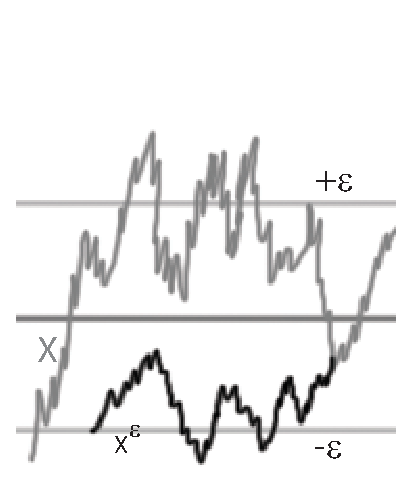
\includegraphics[scale=0.33]{r2dc.eps}} & {} & {} &     \\ \cline{2-6}
\multicolumn{1}{|c|} {} &  \multirow{6}{*}{$\statewebapart$} &  & \multirow{6}{*}{indep.} & \multirow{3}{*}{$\statenoweb$} & \multirow{3}{*}{hits   $0$}\\
\multicolumn{1}{|c|} {} & {} & {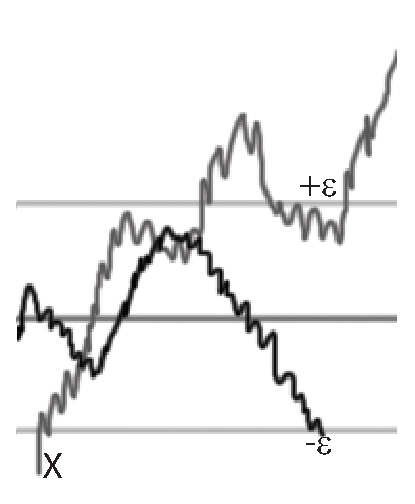
\includegraphics[scale=0.33]{r2dnc.eps}} & {} & \multirow{-3}{*}{$\statewebtogether$} &   \multirow{-3}{*}{hits  $\sampled$}  \\ \cline{2-6}
\multicolumn{1}{|c|} {} & {\multirow{6}{*}{$\statewebtogether$}} & {}& \multirow{6}{*}{equal} & \multirow{6}{*}{$\statewebapart$} & \multirow{6}{*}{hits $0$}     \\
\multicolumn{1}{|c|} {} & {} & {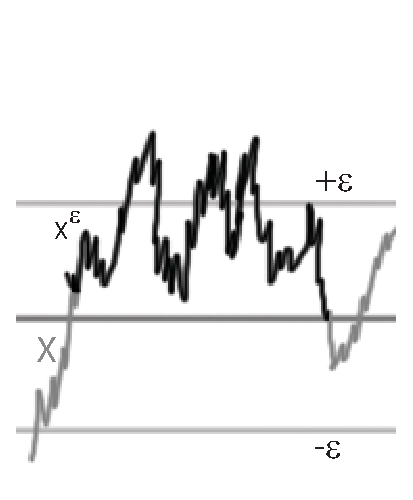
\includegraphics[scale=0.33]{r1d.eps}} & {} & {} &      \\ \hline\hline %\cline{1-6}
\multicolumn{1}{|c|}{\multirow{20}{*}{$\twodim=(x,y)$}} &
\multicolumn{1}{|c|} {\multirow{6}{*}{$\statenoweb$}} &  & \multirow{6}{*}{indep.} & \multirow{6}{*}{$\statewebapart$} & \multirow{6}{*}{$x=\pm\epsilon$}     \\
\multicolumn{1}{|c|} {\multirow{10}{*}{$x=\resamplede$}} & {} & {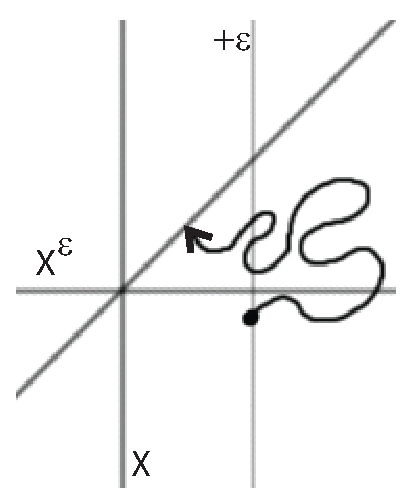
\includegraphics[scale=0.33]{s2dc.eps}} & {} & {} &     \\ \cline{2-6}
\multicolumn{1}{|c|} {\multirow{10}{*}{$y=\sampled$}} &  \multirow{6}{*}{$\statewebapart$} &  & \multirow{6}{*}{indep.} & \multirow{3}{*}{$\statenoweb$} & \multirow{3}{*}{$x=0$}\\
\multicolumn{1}{|c|} {} & {} & {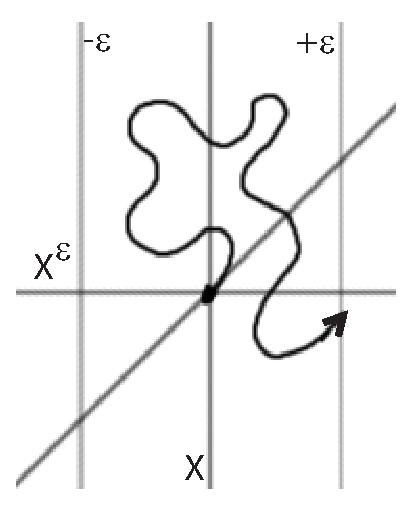
\includegraphics[scale=0.33]{s2dnc.eps}} & {} & \multirow{-3}{*}{$\statewebtogether$} &   \multirow{-3}{*}{$x=y$}  \\ \cline{2-6}
\multicolumn{1}{|c|} {} & {\multirow{6}{*}{$\statewebtogether$}} & {}& \multirow{6}{*}{equal} & \multirow{6}{*}{$\statewebapart$} & \multirow{6}{*}{$x=y=0$}     \\
\multicolumn{1}{|c|} {} & {} & {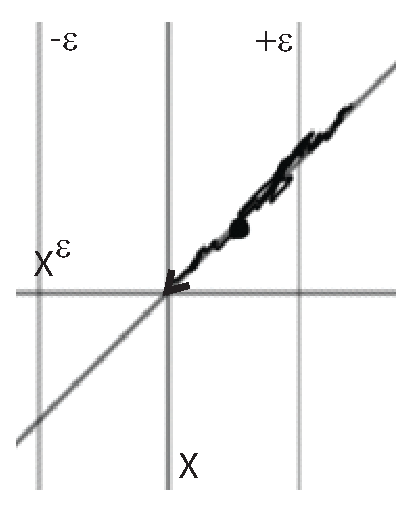
\includegraphics[scale=0.33]{s1d.eps}} & {} & {} &    \\
     \hline
  \end{tabular}
\end{center}
\caption{Illustrated states and transitions of $\twodim$}
\end{figure}
\TODO{}{Break lines in titles of two last columns}

We can now reduce Lemma \ref{lem:resamplede-to-sampled} and rephrase it in terms of $\twodim$:
\begin{lemma*}
$\P(\twodim_t \in \{(x,y) \ :\  |x-y|<\delta \} \text{ for all } t \in [0,1])\to1$ as $\epsilon\to 0$.
\end{lemma*}
The reduction of Lemma \ref{lem:resamplede-to-sampled} to the above
follows from the scale-invariance properties of Brownian motion. Those
imply that proving the convergence uniformly on the interval $[0,1]$
suffices to prove the convergence on every bounded time interval.
\newcommand{\boundarylines}{A}
Fix $\delta>0$, and define $\boundarylines=\{(x,y) \ :\  |x-y|=\delta \}$.
The above lemma can now be rephrased as
\begin{lemma*}
  The probability that before time $1$, $\twodim$ has hit $\boundarylines$
  is $o(1)$.
\end{lemma*}
This lemma can be further reduced to the following:
\newcommand{\farpoint}{(P,P)}
\newcommand{\probhitboundaryis}[1]{Fix $P > 0$.  The probability that $\twodim$
  hits $\boundarylines$ before $\farpoint$ is #1}

\begin{lemma}\label{lem:prob-hit-boundary-o1}
  \probhitboundaryis{$o(1)$}
\end{lemma}

\newcommand{\origin}{(0,0)}

\begin{proof}[The reduction proceeds as follows:]

  Let $\eta > 0$.

  Choose $P$ so that the probability that standard Brownian motion
  travels from $0$ to $P$ in time less than $1$ is less than
  $\eta$.

  Choose $\epsilon$ such that the probability that $\twodim$ hits
  $\boundarylines$ before $\farpoint$ is less than $\eta$.

  Then the probability that $\twodim$ hits $\boundarylines$ before $\farpoint$
  or takes less time than $1$ to return from $\farpoint$ to $\origin$ is
  less than $2\eta$.

  \FIXME{}{There needs to be some mention of time scaling here}
\end{proof}

In summary, we have reduced Lemma \ref{lem:resamplede-to-sampled} to
Lemma \ref{lem:prob-hit-boundary-o1}. We prove the latter in the
following section using the notion of excursions of $\twodim$.

\subsection{Excursions of $\twodim$}

\newcommand{\excursionstart}{T}
{
  Almost surely, the times at which $\twodim = 0$ (which are stopping
  times) form an infinite discrete collection $\excursionstart_0 <
  \excursionstart_1 < \cdots$. We say ``the probability that an excursion
  hits a set $X$ is $p$'', if $\P(\twodim_t\in X \text{
  for some } t\in [\excursionstart_0, \excursionstart_{1}]) = p$.

  Observe that by equidistribution the probability is the same when
  $t$ ranges over $[\excursionstart_i, \excursionstart_{i+1}]$, and
  note that the hitting events in question are independent.
}

\newcommand{\probexcursionhits}[1]{\P\left(\text{an excursion hits #1}\right)}

Using this definition we can now use the following strategy to
prove Lemma \ref{lem:prob-hit-boundary-o1}:
\[
\frac{\probexcursionhits{\boundarylines}}
     {\probexcursionhits{\farpoint}}
        \to 0 \text{ as } \epsilon\to0
\]
As the hitting events on different excursions are independent we
can deduce it is much more likely that hitting $\farpoint$ happens
before hitting $\boundarylines$. This implies Lemma
\ref{lem:prob-hit-boundary-o1}. This philosophy is
realized through the next couple of lemmas.

\newcommand{\Omegaeloge}{\Omega(\epsilon\log\epsilon)}

\begin{lemma}
  \label{lem:Phitboundaryline}
  $\probexcursionhits{\boundarylines}$ is $O(\epsilon)$.
\end{lemma}

\begin{lemma}
  \label{lem:Pabsorbedandtravelsfar}
  For any fixed $P > 0$, $\probexcursionhits{\farpoint}$ is $\Omegaeloge$.
\end{lemma}

We are now in a position to prove something slightly stronger than
Lemma \ref{lem:prob-hit-boundary-o1}.

\begin{lemma}\label{lem:prob-hit-boundary-o1loge}
  \probhitboundaryis{$O(\frac{1}{\log\epsilon})$}
\end{lemma}

\newcommand{\Oe}{O(\epsilon)}

\begin{proof}
  $\twodim$ consists of a sequence of excursions, each of which satisfies
  exactly one of the following conditions
  \begin{itemize}
  \item the excursion hits $\boundarylines$ (with probability
    $O(\epsilon$))
  \item the excursion does not hit $\boundarylines$ but does hit
    $\farpoint$ (with probability $\Omegaeloge-\Oe$, which is itself
    $\Omegaeloge$)
  \item the excursion does not hit $\boundarylines$ or $\farpoint$ before
    returning to $\origin$
  \end{itemize}
  When $\twodim$ returns to $\origin$ a new excursion begins, which is independent of
  the previous excursions.  Thus the probability that the first
  condition occurs before the second is exactly the probability of the
  first as fraction of the sum of their probabilities, that is
  \[
  \frac{\Oe}{\Omegaeloge + \Oe} = O\left(\frac{1}{\log\epsilon}\right)
  \]
\end{proof}

We conclude by providing the proofs of the two previously
stated lemmas.

\subsection{Proofs of the excursion lemmas}
\newcommand{\tdh}{\rotproc^1}
\newcommand{\tdv}{\rotproc^2}
\newcommand{\rotproc}{Z}

In this section we give the proof of Lemmas \ref{lem:Phitboundaryline}
and \ref{lem:Pabsorbedandtravelsfar}.
For convenience we rotate (and scale) $\twodim=(\twodim^1,\twodim^2)$, defining
$\rotproc=(\tdh,\tdv)=(\twodim^1+\twodim^2,\twodim^1-\twodim^2)$.

\begin{proof}[Proof of Lemma \ref{lem:Phitboundaryline}]
Consider the process $\twodim$ between times $\excursionstart_0$ and $\excursionstart_1$.
Our goal is to show that with probability at least $1-o(\epsilon)$, $\twodim$ arrives in
$\statewebtogether$, before hitting $\boundarylines$. That is because once it arrives at
$\statewebtogether$ it can never hit $\boundarylines$ before hitting $\origin$.
We now show to following two
auxiliary claims:

\begin{claim}
 Whenever $\tdv=0$ the probability that subsequently $\twodim$ arrives at $\statewebtogether$ before $\tdv$ hits $\epsilon$ is at least a constant (independent of $\epsilon$).
\end{claim}

\begin{claim}
Whenever $\tdv=\pm\epsilon$ then with probability at least $\epsilon/\delta$ of $\tdv$ hitting $0$ before it hits $\pm\delta$.
\end{claim}

Claim 1 follows from scale invariance, while Claim 2 is a standard martingale result on Brownian motion (observing that on the relevant time interval $\tdv$ is a standard Brownian motion).

The reduction of Lemma \ref{lem:Phitboundaryline} to those two claims is similar to the
proof of Lemma \ref{lem:prob-hit-boundary-o1loge}. Claims 1 and 2 imply that between two consecutive times when $\tdv=0$
the ratio of the probability of $\twodim$ arriving at $\statewebtogether$ and the probability
of it hitting $\boundarylines$ tends to $0$. We can now deduce Lemma \ref{lem:Phitboundaryline} from the fact that the behavior of $\twodim$ is independent on those intervals.
\FIXME{}{Make this paragraph clearer}
\end{proof}

\begin{proof}[Proof of Lemma \ref{lem:Pabsorbedandtravelsfar}]
We bound below the probability that an excursion hits $\farpoint$,
i.e.\ $\rotproc$ hits $(P,0)$ before returning to $\origin$.

After a stopping time at which $\twodim = \rotproc = \origin$ there is a positive probability $C$
that $\rotproc$ hits $Q=[0, \epsilon] \cross
\{\epsilon\}$ before returning to $\origin$.
By scale invariance $C$ is independent of $\epsilon$.

Let $(x,\epsilon)\in Q$ and consider $\rotproc$ after hitting $(x,\epsilon)$.
We calculate the hitting density of this process on the horizontal axis.
By the classical result on the hitting density on a line of the two-dimensional
Brownian motion, this density for points on $L^+$ is at least
\[
K\frac{1}{\epsilon} \frac{1}{1 + (y/\epsilon)^2} dy
\]
where $K$ is a normalizing constant (independent of $\epsilon$).

By the same martingale argument used above, after hitting a point $(x,0)$ the
probability of hitting $(P,0)$ before $\origin$ is $x/P$ for all $0\le x\le P$.
Integrating this against the hitting density we get that the probability that
$\rotproc$ started from some point in $Q$ hits $L^+$
between $\epsilon$ and $1$ and then travels to $\farpoint$ before returning
to $\origin$ is at least
\[
\frac{K}{P} \int_{\epsilon}^{1} \frac{y/\epsilon}{1 + (y/\epsilon)^2}
\, dy
\]
which is
\[
\frac{K\epsilon}{2P} \log\left(\frac{1 + (1/\epsilon)^2}{2}\right)
\]
which is $\Omegaeloge$.
\end{proof}
}
